% ================
% Landon Buell
% Qioayan Yu
% GLSVLSI'2020
% 16 June 2020
% ================

\documentclass[12pt,letterpaper]{article}

\usepackage{float}
\usepackage{graphicx}
\usepackage{subfigure}
\usepackage{amsmath}
\usepackage{amssymb}
\usepackage[left=2.5cm,right=2.5cm,top=2.5cm]{geometry}

\begin{document}


% ================================================================

\section*{Experiment}

\paragraph*{}This case study serves as an experiment in determining how approximate computation techniques may change the performance of a multilayer perceptron (MLP) neural network classifier. We have chosen to a subsection of the MNIST data set containing 28 x 28 pixel images of handwritten digits, each labeled according the digit that appears in the image. Each pixel is given by an integer $0$ through $255$ which indicates the gray-scale value. In the case of each image sample, the digit was known to be roughly centered in the figure. Examples of a few images can be found below in fig. (\ref{images}) . From the full data set, the first $10,000$ images were chosen to train each model, and the next $6,000$ were chosen to test the model.

\paragraph*{}Given that each image is centered in a given sample, we propose that approximating a border of pixels around the outside of the image would produce small changes in the performance of the classifier model, given that dominant features would be preserved. To apply this approximation, we tested a baseline set of samples against samples that have varying depth pixel borders that have been approximated. This effectively creates a padding  $3$, $5$, or $7$ pixels on each image. Each approximated pixel value was transformed from a byte to a double precision floating-point number, where the most-significant-bit in the float's exponent was forces to $0$, thus only allowing those pixels to exist in the closed interval $[-1,+1]$.

\begin{figure}[h]
	\centering
	\subfigure[]{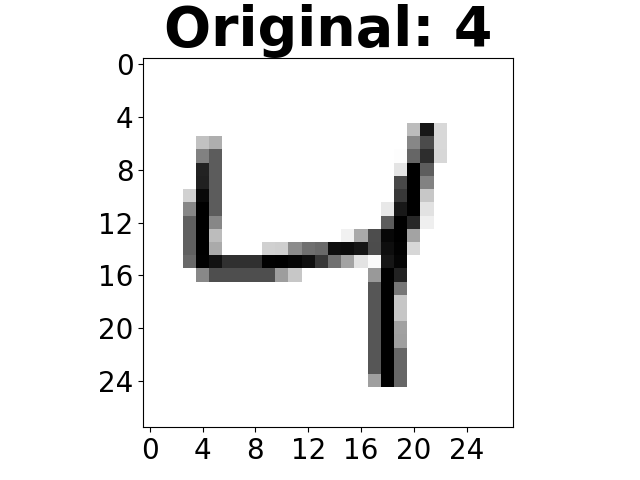
\includegraphics[width=0.45\columnwidth]{Original_4}}
	\subfigure[]{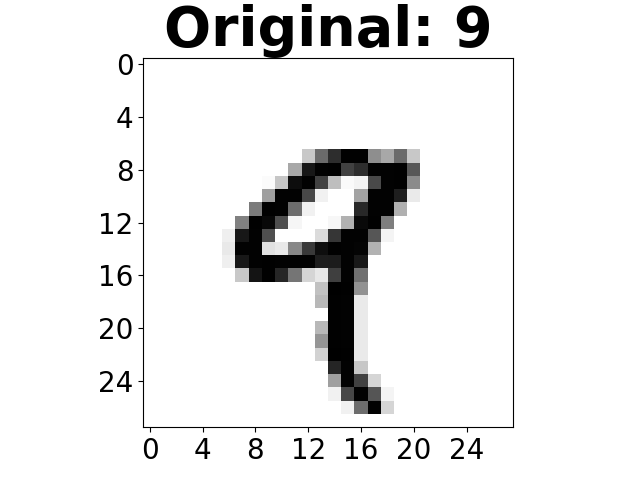
\includegraphics[width=0.45\columnwidth]{Original_9}}	
	\subfigure[]{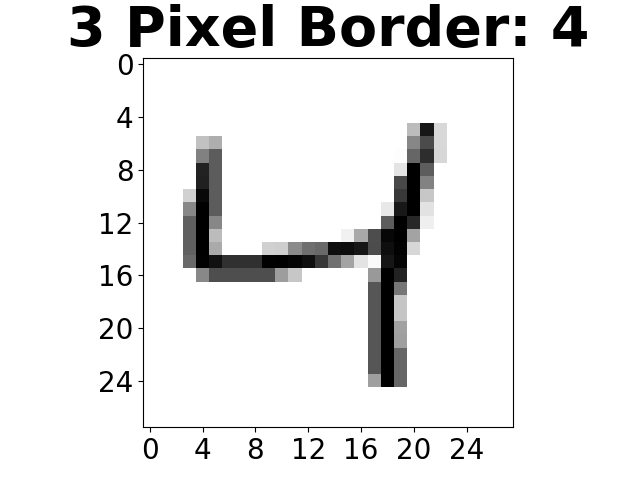
\includegraphics[width=0.45\columnwidth]{3_Pixel_Border_4}}
	\subfigure[]{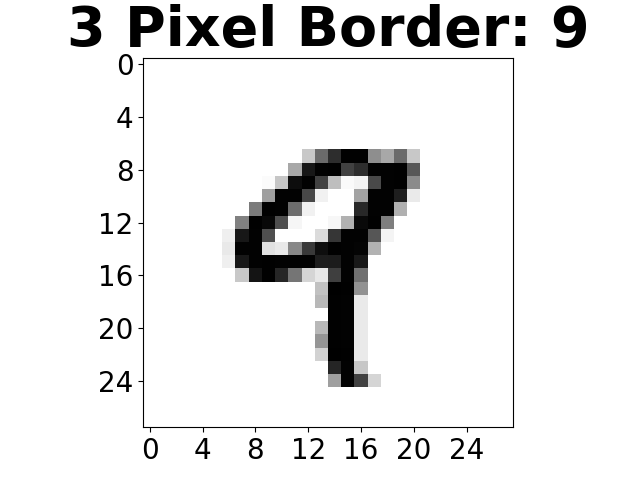
\includegraphics[width=0.45\columnwidth]{3_Pixel_Border_9}}	
	\subfigure[]{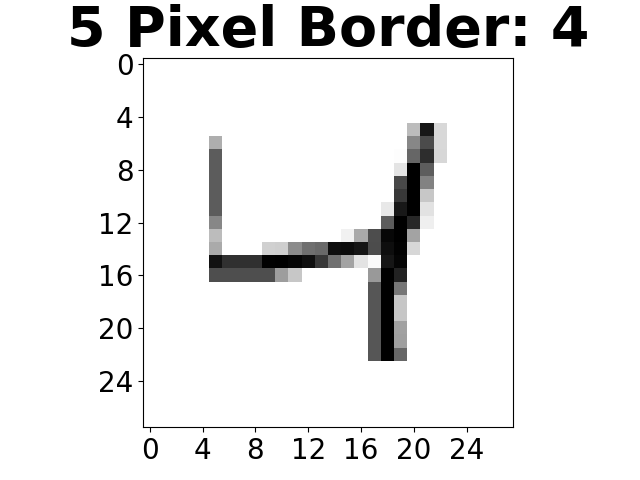
\includegraphics[width=0.45\columnwidth]{5_Pixel_Border_4}}
	\subfigure[]{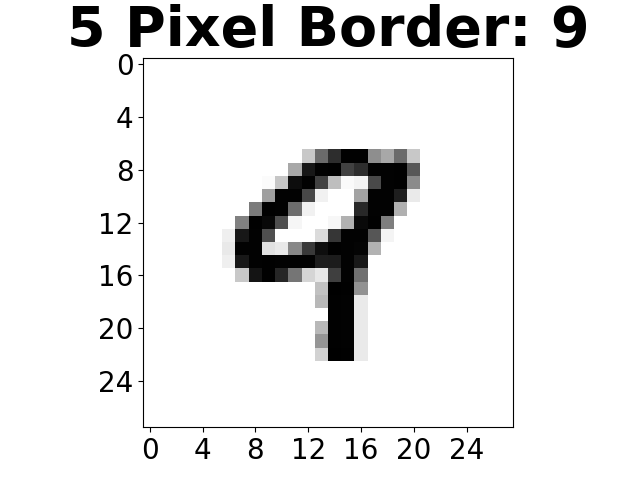
\includegraphics[width=0.45\columnwidth]{5_Pixel_Border_9}}	
	\subfigure[]{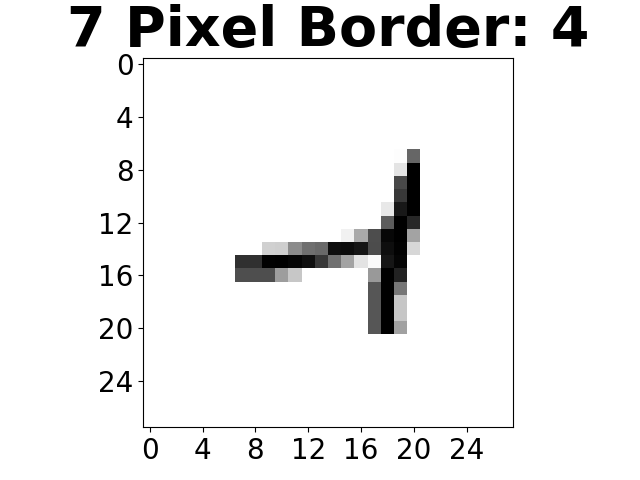
\includegraphics[width=0.45\columnwidth]{7_Pixel_Border_4}}
	\subfigure[]{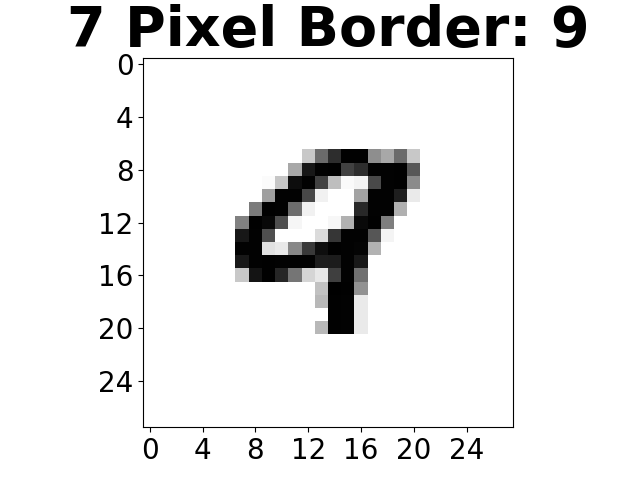
\includegraphics[width=0.45\columnwidth]{7_Pixel_Border_9}}			
	\caption{Digit Samples showing how approximating a border of bits around each images affects the figure. When darker pixels are approximated, the become white.}
	\label{images}
\end{figure}

\paragraph*{}For some samples, it can be seen that even approximating a large border of pixels, the characteristics of the digit are preserved, see fig.\ref{images}(h). For other samples, characteristic information man be lost and lead to classification errors, see fig. (\ref{images}g). Each training ans testing set of digit images was given to different MLP architecture variants. We adjusted the hidden layers to contain $20$, $40$, $60$, $80$, $100$, and $120$ neurons per layer, for one and two hidden layers. $10$ training epochs were used in all cases, with batch sizes of $100$ samples used in each step for a Stochastic Gradient Descent Optimizer.

% ================================================================

\section*{Conclusion}

\begin{figure}[h]
	\centering
	\subfigure[]{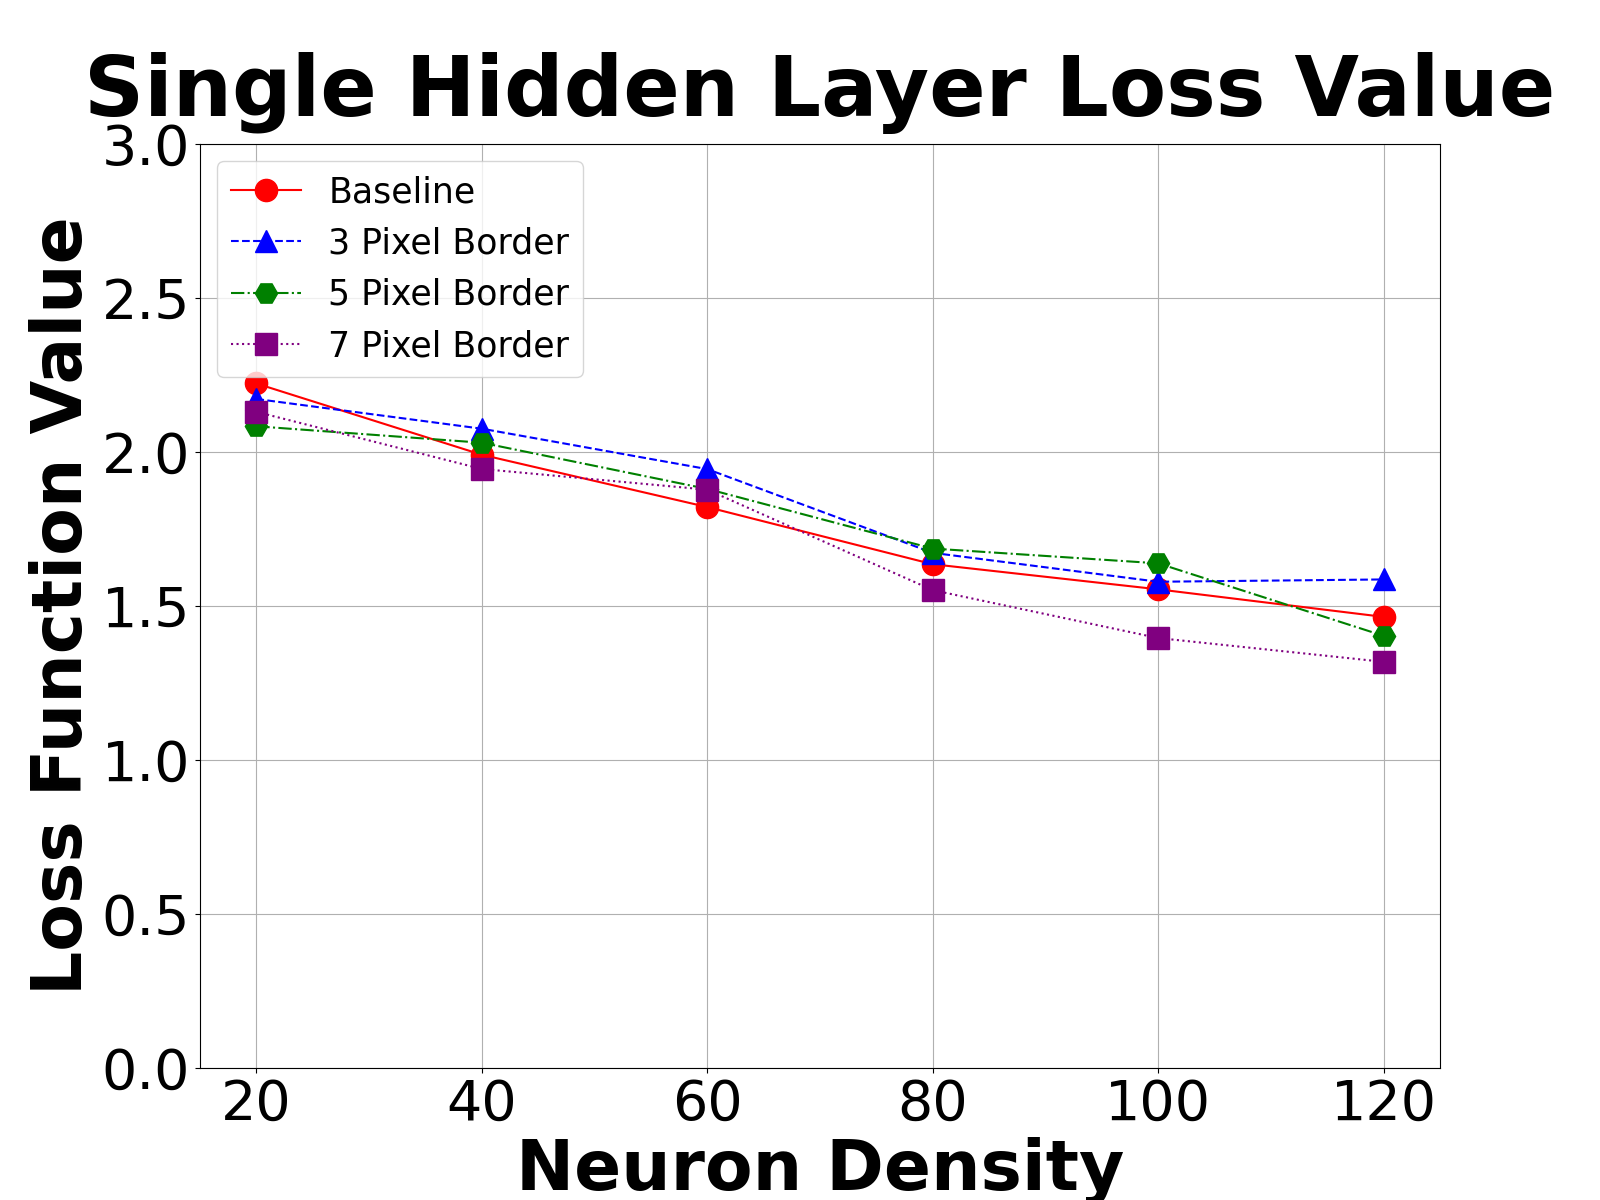
\includegraphics[width=0.45\columnwidth]{Single_Hidden_Layer_Loss_Value_approx}}
	\subfigure[]{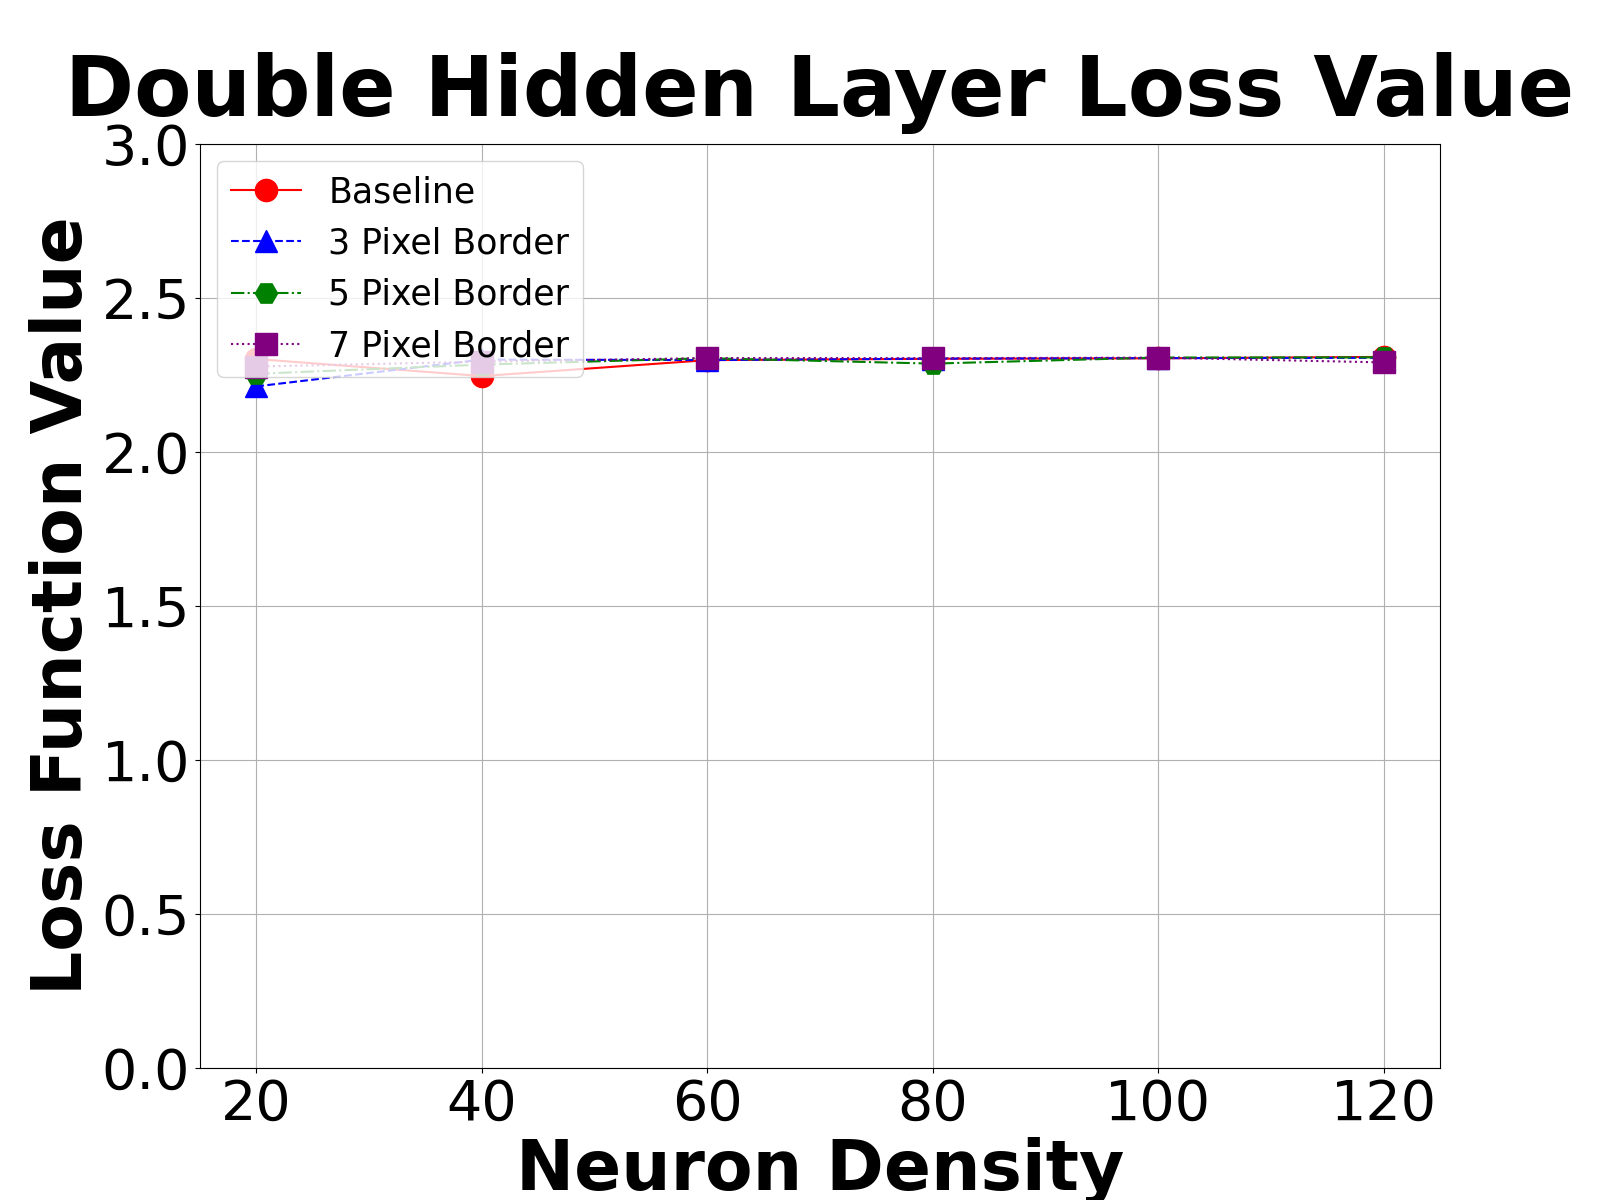
\includegraphics[width=0.45\columnwidth]{Double_Hidden_Layer_Loss_Value_approx}}
	\subfigure[]{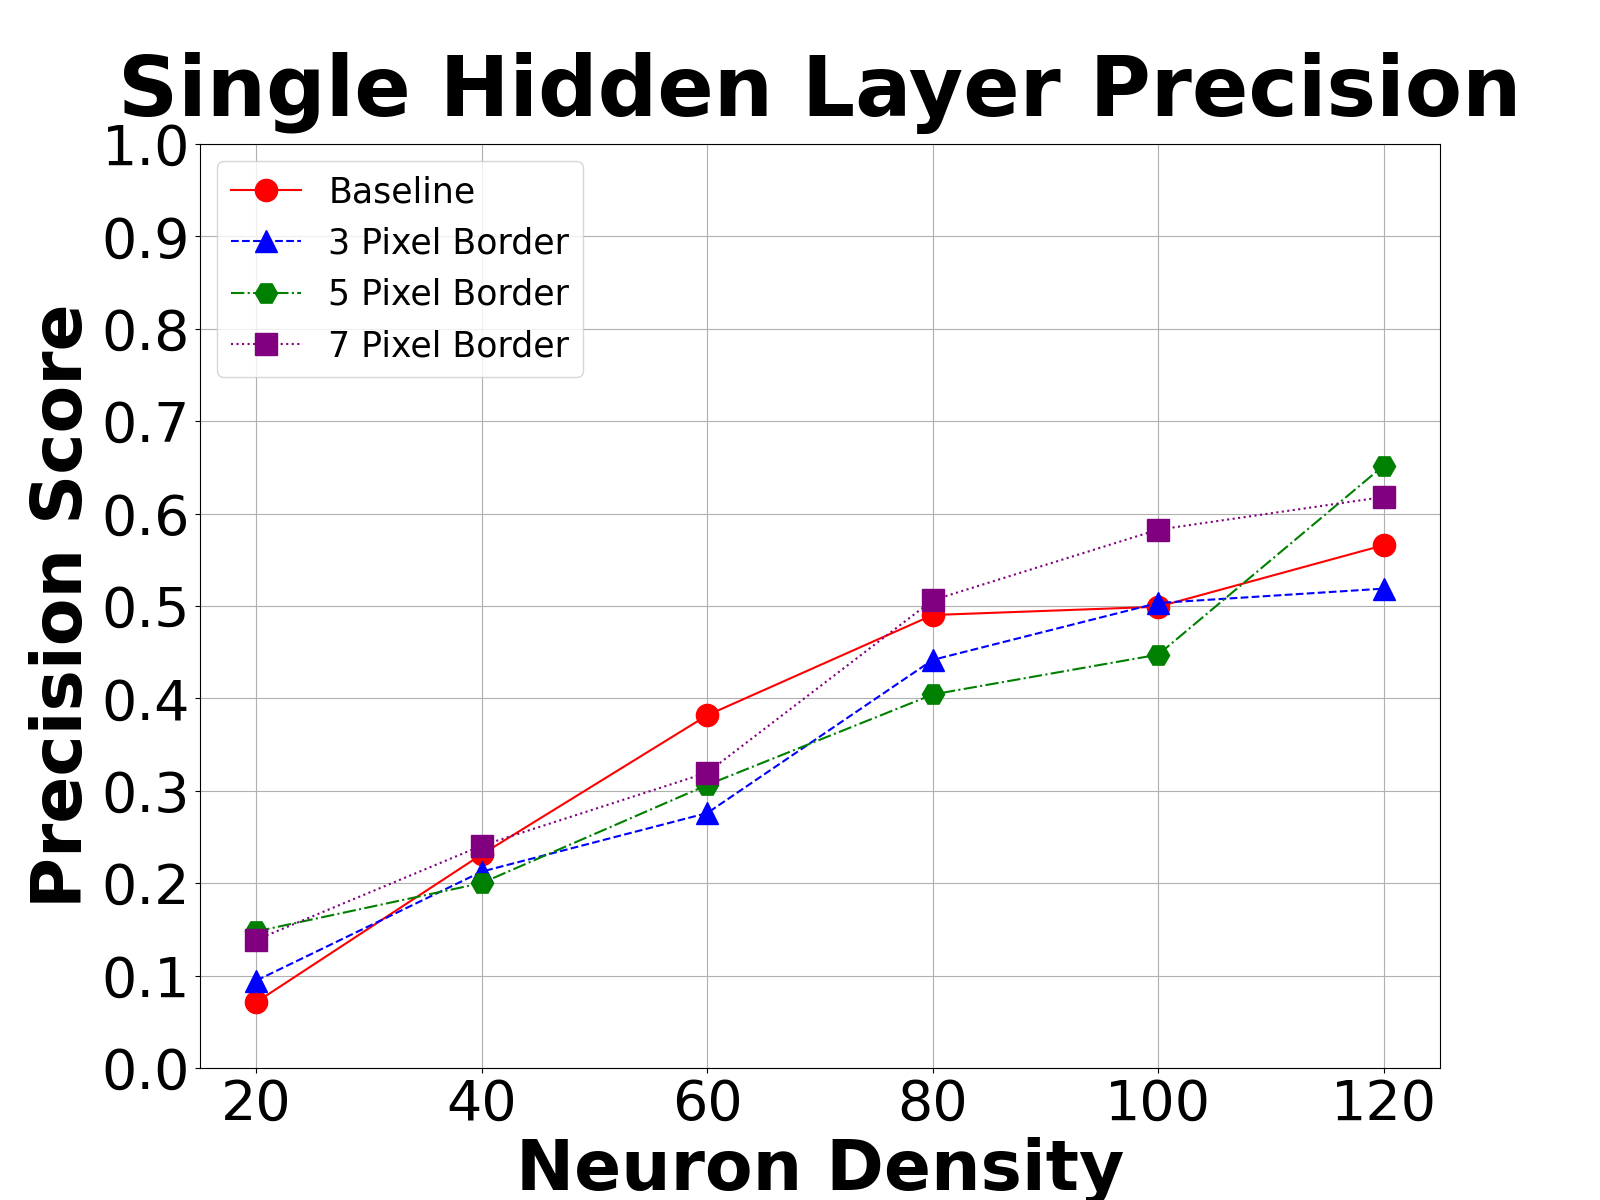
\includegraphics[width=0.45\columnwidth]{Single_Hidden_Layer_Precision_approx}}
	\subfigure[]{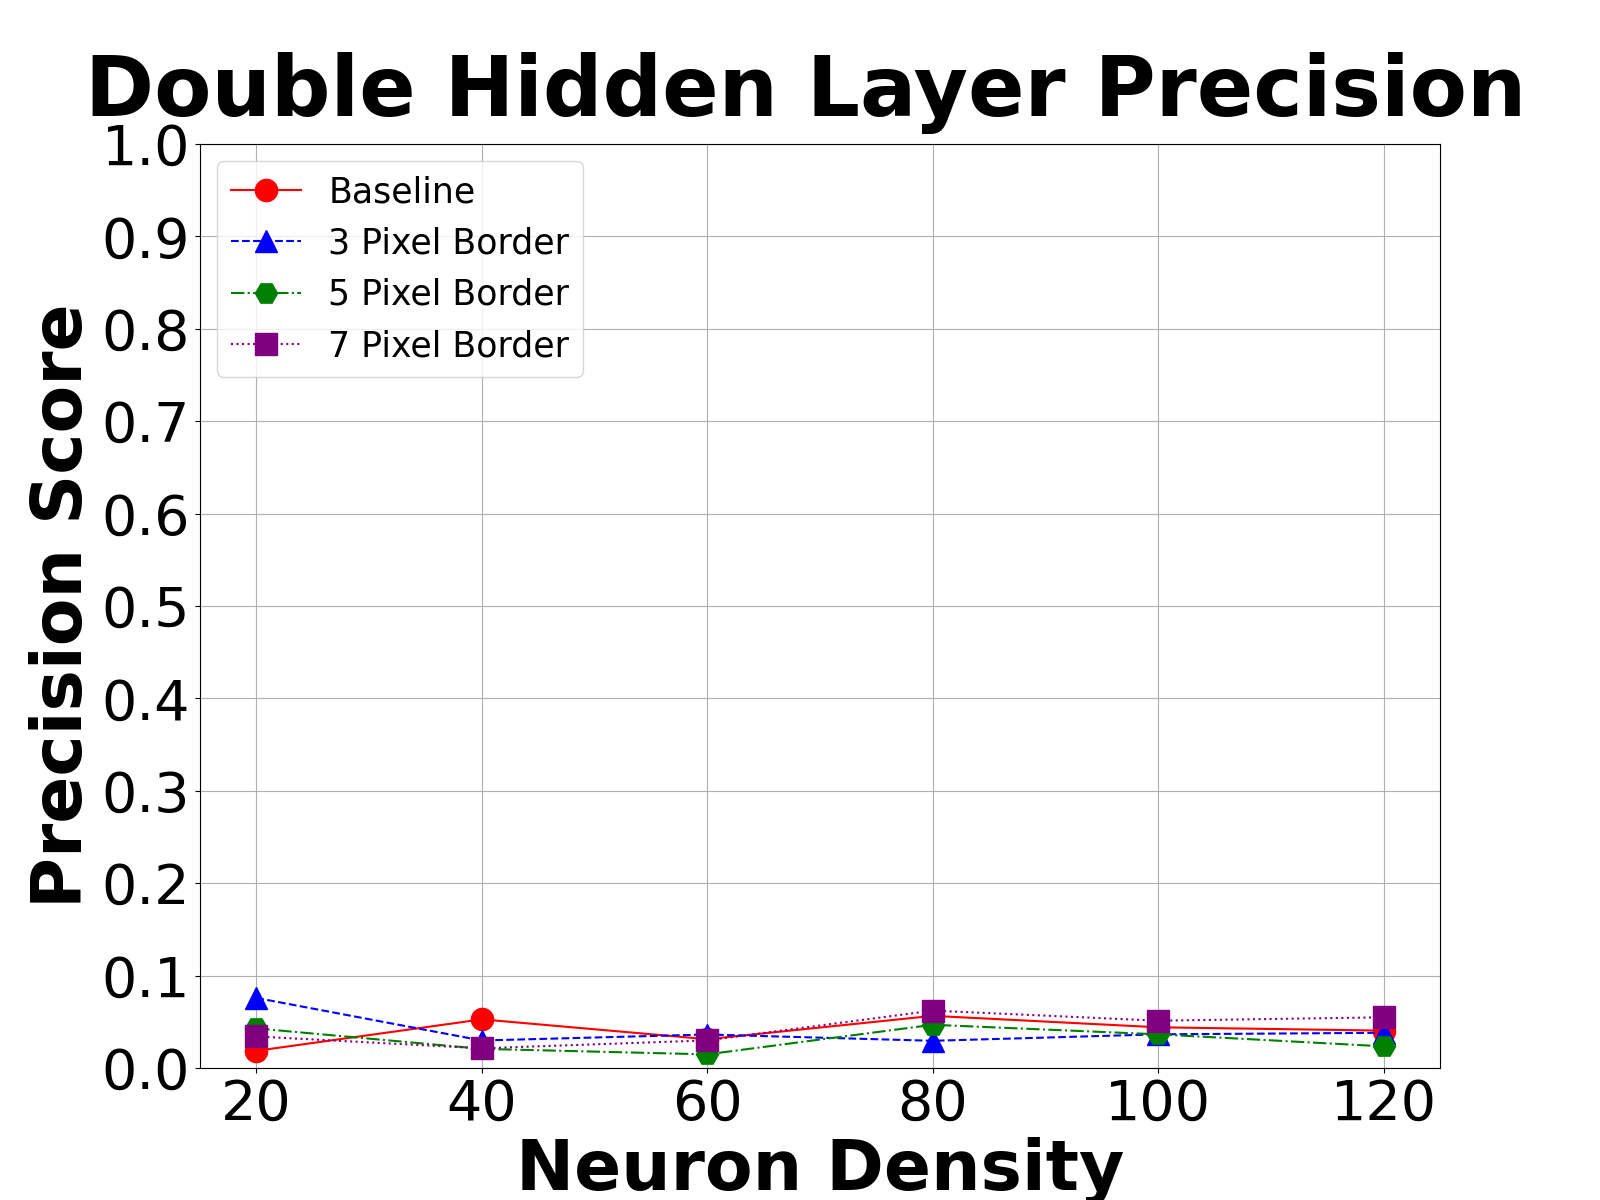
\includegraphics[width=0.45\columnwidth]{Double_Hidden_Layer_Precision_approx}}
	\subfigure[]{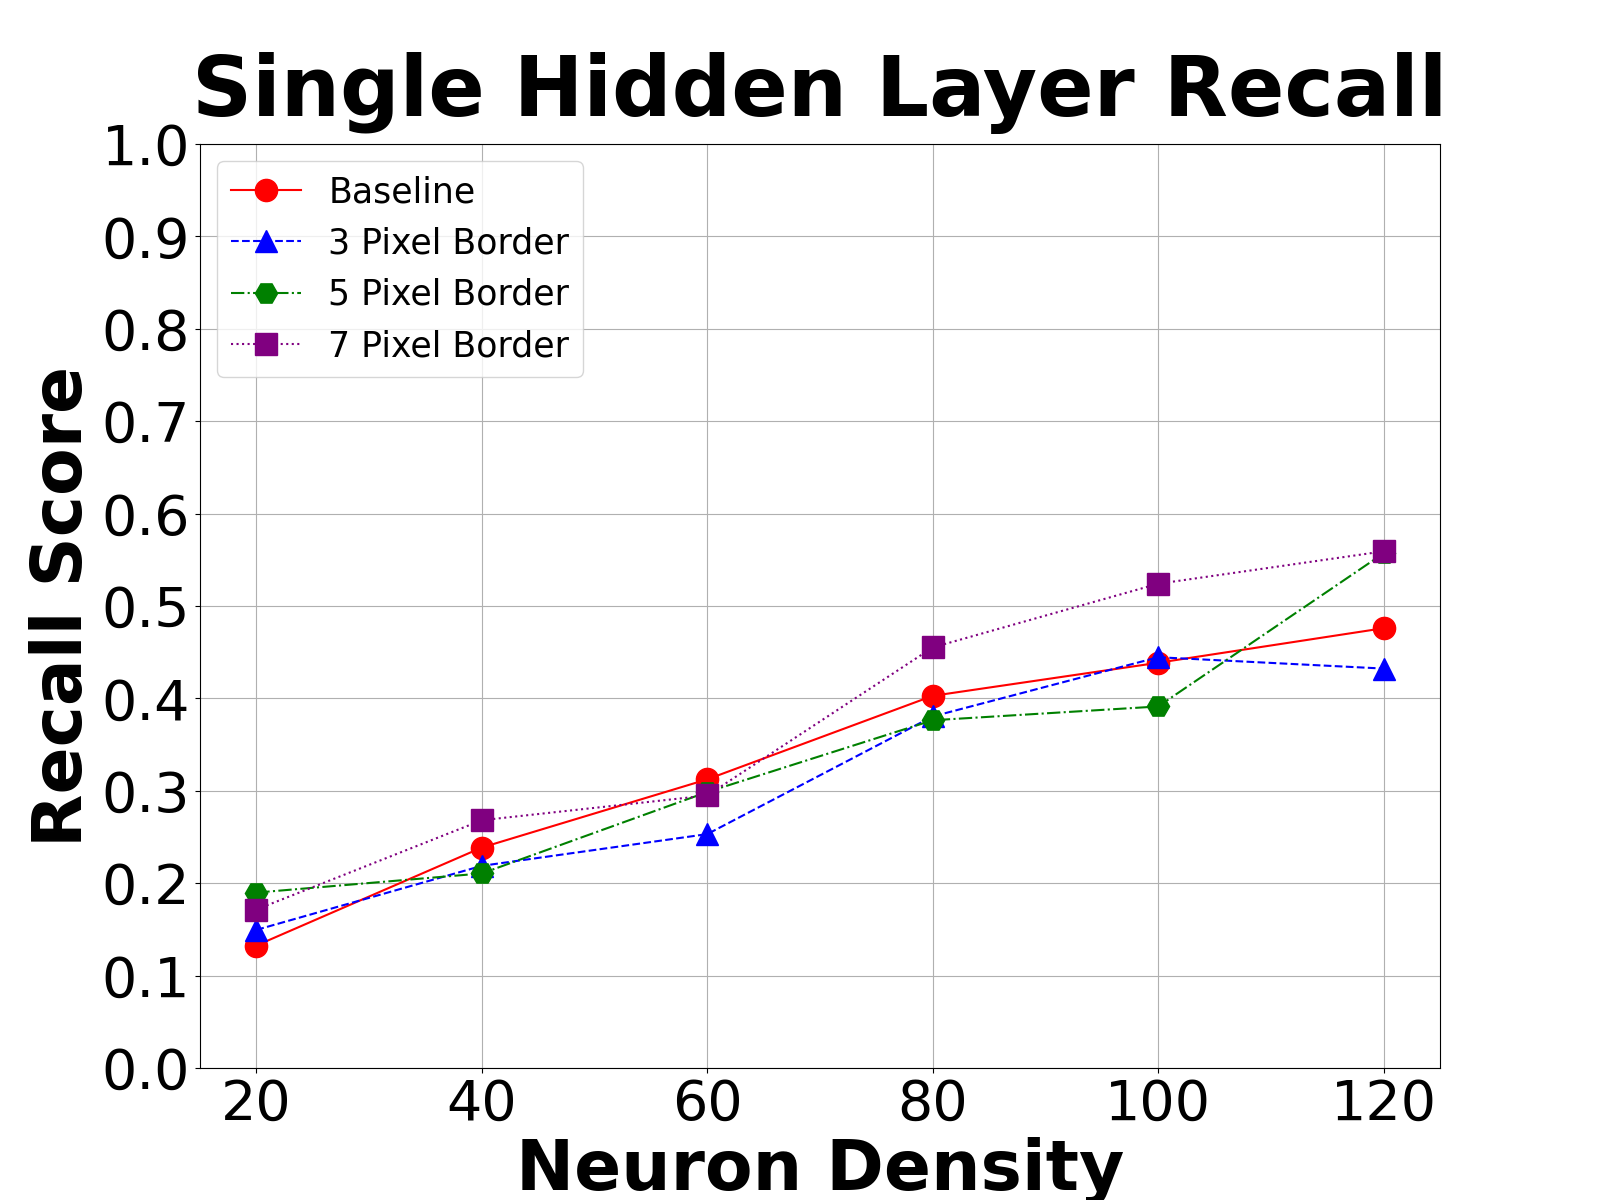
\includegraphics[width=0.45\columnwidth]{Single_Hidden_Layer_Recall_approx}}
	\subfigure[]{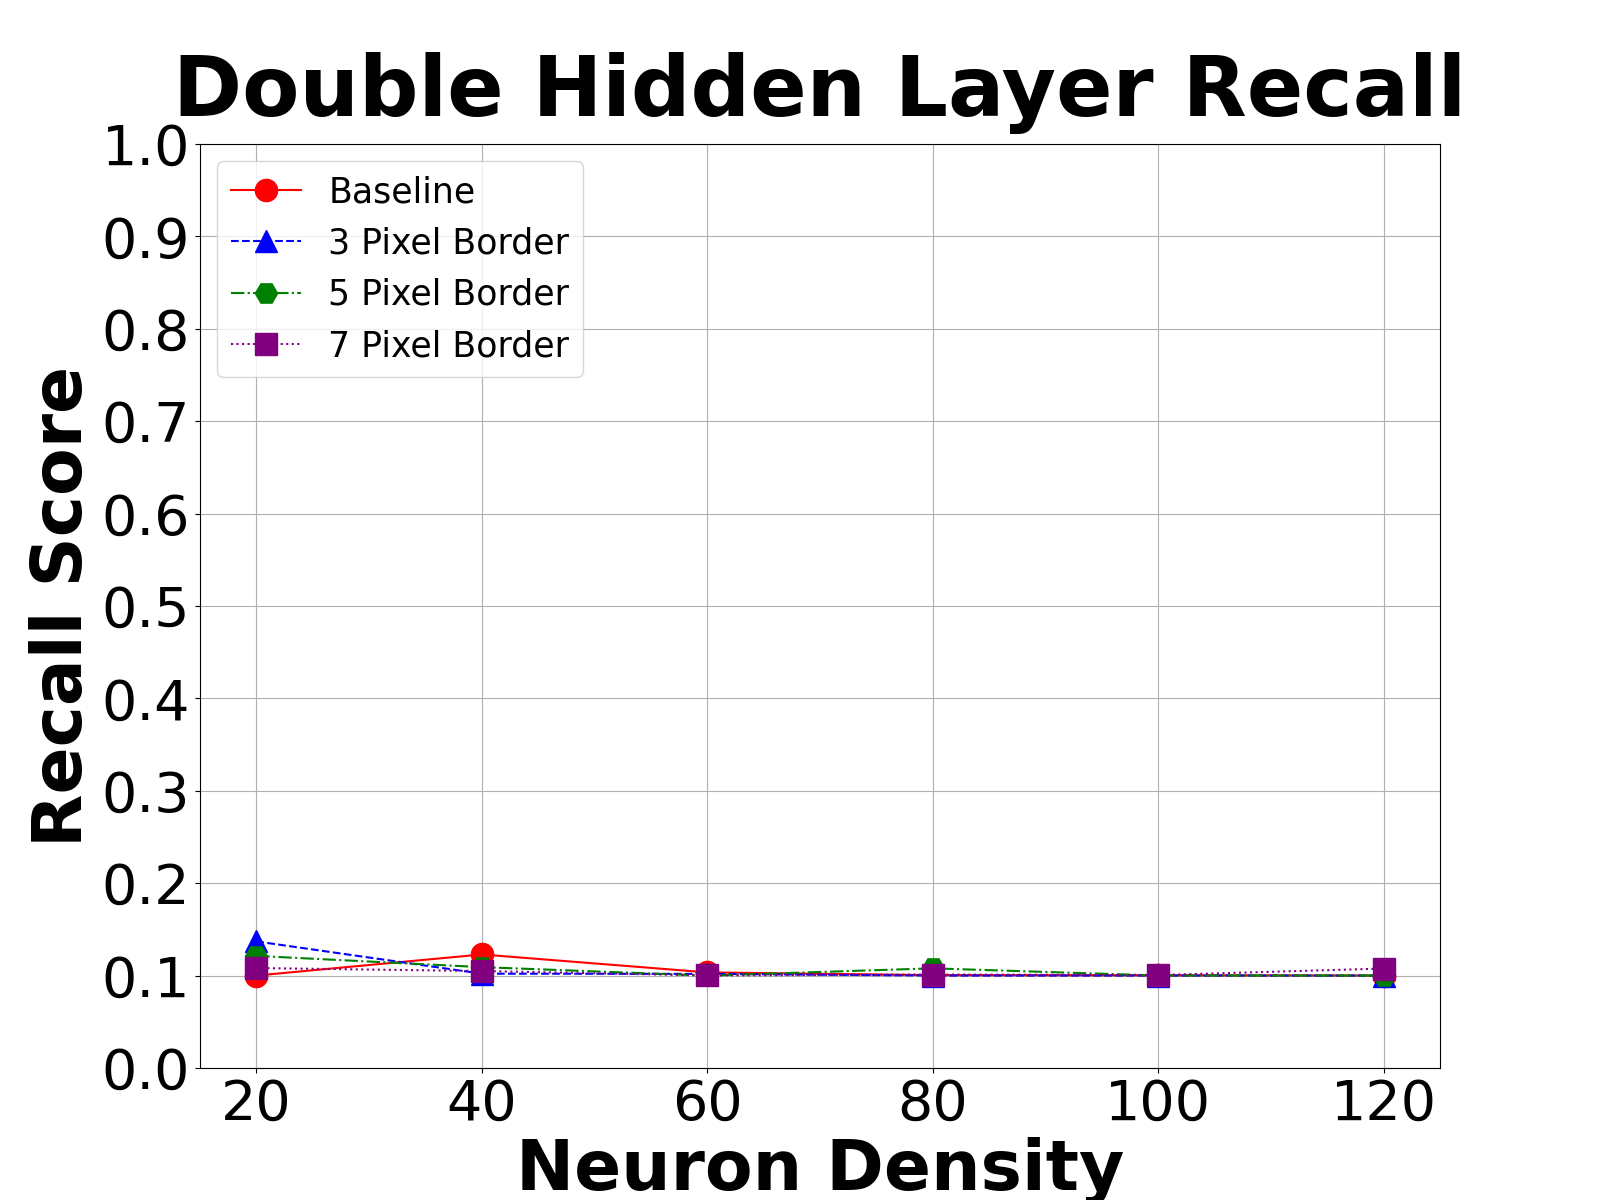
\includegraphics[width=0.45\columnwidth]{Double_Hidden_Layer_Recall_approx}}
	\caption{Experimental results for baseline and $3$, $5$, and $7$ approximated pixel padding border. The same approximations were applied to all samples in both training and testing sets. All data points are taken from the average of 10 models with identical hyper parameters, and non-identical initial weight parameters.}
	\label{results}
\end{figure}

\paragraph*{}The preliminary results of this experiment, for one and two hidden layers, over the selected set of neuron densities shows that applying a $3$, $5$, and $7$ border of approximated pixels presents no major deviation in performance from the baseline models. In fig. (\ref{results}a) and (\ref{results}b), the consistency between training and test samples shows no discernible changes in the loss function. This means that while a subset of pixels were approximated the dominant features preserved in the center of the figure still allowed the optimization process to converge on a similar set of parameters as the baseline samples.

\paragraph*{}Similarly, the classification of previously unseen samples, as judged by each model's classification precision (\ref{results}c. , \ref{results}d.) and recall (\ref{results}e. , \ref{results}f.) scores also differs very slightly from the baseline.  Due the relatively small volume of training training data and such few epochs, these score ranks low across all models, and particularly low as the network depth increases from a single hidden layer to two hidden layers. However the small change in performance from the baseline indicates that characteristic features are preserved, and the overall performance of the model remains consistent, even with a border of approximated pixels.


% ================================================================

\end{document}